% Oliver Chi, draft for research project
% 1/9/2018
%
\documentclass[runningheads]{llncs}
%
\usepackage{graphicx}
\usepackage{amsfonts}
\usepackage[linesnumbered,lined,boxed,commentsnumbered]{algorithm2e}
\usepackage[utf8]{inputenc}
\usepackage{amsmath}
\usepackage{mathtools}
\usepackage{enumitem}
\makeatletter
\makeatother
%
%
%
%
\begin{document}
%
\title{Transfer Learning for Depression Detection on Social Networks\thanks{Supported by School of Information System, University of Southern Queensland, Australia}}
%
%
\author{Oliver Chi\inst{1}\and
Xiaohui Tao\inst{1} }
%
%
\institute{School of Information System, University of Southern Queensland, Australia\\
\email{\{ochi,xtao\}@usq.edu.au}}
%
\maketitle
%
\begin{abstract}
The abstract should briefly summarize the contents of the paper in
150--250 words.
%
\keywords{psychological knowledge base \and ensemble classification technique \and supervised learning \and depression.}
\end{abstract}
%
%
%
%
%
%
%
%
%
%
%
%
%
%
%
%
%
%
%
%
%
%
\pagebreak
\section{Introduction}
%
%
%
%
%
%
%
%
%
%
%
%
%
%
%
%
%
%
%
%
%
%
\pagebreak
\section{Related Work}
%
%
\subsection{Psychological Studies}
%
%
\subsection{Classification Research on Depression}
%
%
%
%
%
%
%
%
%
%
%
%
%
%
%
%
%
%
%
%
%
\pagebreak
\section{Definitions/Research Problem}
%
%
\paragraph{}
.... The research objective is defined:\\
\textbf{Definition 1} \textit{Let $\mathbb{S}$ be a set of user properties to present an effective user profile for depression, a user property s $\in$ $\mathbb{S}$ is a tuple $s := \langle p_{1}, p_{2}, p_{3}$, $\cdots p_{n} \rangle$, where
\begin{itemize}
  \item p is a visualisation or instance of an user property;
  \item p is not a mental or depression close-related symptom;
  \item n could be an infinite integer so the number of p elements could be unlimited;
  \item all p elements in the same user profile are generally independent.
\end{itemize}
}
%
%
\paragraph{}
With clear definition of research objective, the research target is defined:\\
\textbf{Definition 2} \textit{Let $\mathbb{V}$ be a set of labeled user depression, a label of user depression v $\in$ $\mathbb{V}$ is a screening result of personal depression, where
\begin{itemize}
  \item when v is binary, it presents depression (1) or healthy (0);
  \item when v is scale, it presents the severity of depression from healthy (0) to most severe depression(1).
\end{itemize}
}
%
%
\paragraph{}
From Definition 1, any given user property s $\in$ $\mathbb{S}$ is possibly overlapped with other user properties. The overlapped information in user profile apparently doesn't suit for classification. While learning from related psychological researches, a set of user personal functionings can present a perfect reflection of user mental profile. 
It innovates a creative method that detecting user depression by analysis of a set of user functionings. Therefore, the research problem is defined:\\
\textbf{Definition 3} \textit{Let $\mathbb{U} = \langle u_{1}, u_{2}, u_{3}$, $\cdots u_{k} \rangle$ be a subset of $\mathbb{S}$, any element u $\in \mathbb{U}$ is a tuple $u := \langle p'_{1}, p'_{2}, p'_{3}$, $\cdots p'_{n'} \rangle$,where
\begin{itemize}
  \item $\mathbb{U}$ is a machine-learning descriptive subset transferred from $\mathbb{S}$ in psychological domain descriptive;
  \item every p' $\in$ u is assigned from a instance p $\in$ s in Definition 1;
  \item $|\mathbb{D}^s|$ is limited due to the limited functionings defined in psychological domain.
\end{itemize}
This research aims to discover an effective classification model $\mathbb{M}$ which provides a reliable mapping of a well-defined $\mathbb{U}$ into $\mathbb{V}$:} \\
\begin{center}
	$\mathbb{U}$ $\xRightarrow{\mathbb{M}}$ $\mathbb{V}$  or  $\mathbb{M}$($\mathbb{U}$) = $\mathbb{V}$
\end{center}
%
%
\paragraph{}
%
%
%
%
%
%
%
%
%
%
%
%
%
%
%
%
%
%
%
%
\pagebreak
\section{Framework}
%
%
Therefore, the research problem is decomposed into two tasks: 
\begin{enumerate}
  \item data processing;
  \item modelling.
\end{enumerate}
%
%
%
%
%
%
%
%
%
%
\subsection{Conceptual Design}
%
%
whole framework
%
transfer knowledge:
data processing:
ensemble and modelling:
%
design standards, outcome
%
%
Driven by the processing of tasks, the conceptual framework of the proposed approach is designed consisting of three modules, as illustrated in Fig.~\ref{fig1}.
\begin{figure}[h]
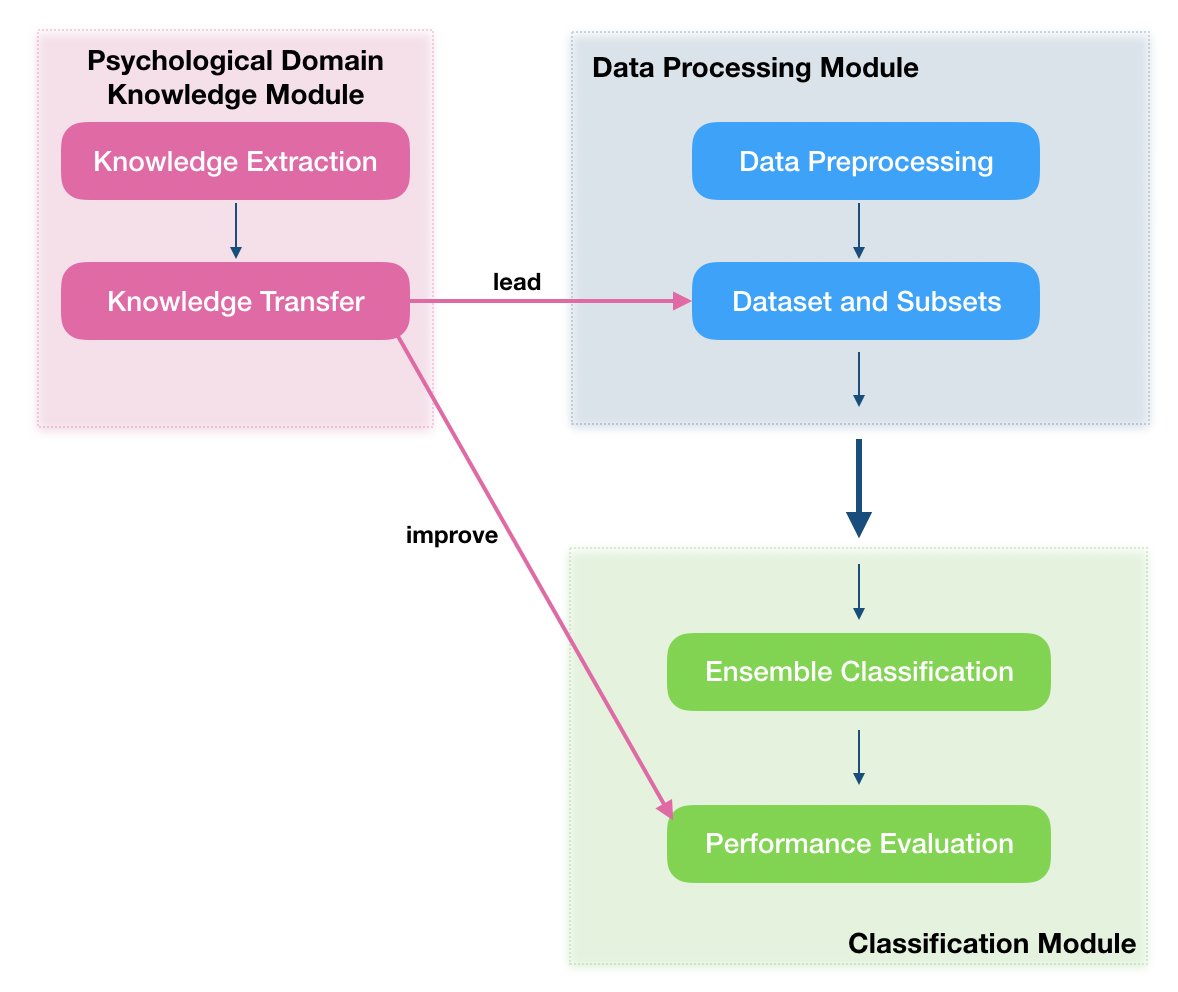
\includegraphics[width=1\textwidth]{concepts.png}
\caption{Conceptual Framework} \label{fig1}
\end{figure}
%
%
%
%
%
%
%
%
%
%
%
\subsection{Psychological Knowledge Base}
%
\paragraph{4.2.1 Psychological Domain Knowledge}
Kroenke et, al. [PHQ-9] concluded that there was a strong association between increasing depression severity screen scores and worsening functionality on all 6 function: mental, social, role, pain, physical and overall functions. Other psychological researchers [Résibois][Stegenga][Xiao, Yoon] also delivered similar opinion on the relation between depression and functions. 
%
\paragraph{4.2.2 Transfer Domain}
We hence can transfer psychological domain knowledge to information domain. \textit{$|\mathbb{D}^s|$} can be narrowed down to 6. The dataset of user mental profile is redefined:\\
\textbf{Definition 4} \textit{ Let new redesigned $\mathbb{U}$ = $\langle u_{mental}, u_{social}, u_{role}, u_{pain}, u_{physical}, u_{overall} \rangle$, every u  $\in \mathbb{U}$ is an independent function of user, where
\begin{itemize}
  \item $u_{mental}$ presents mental function;
  \item $u_{social}$ presents social function;
  \item $u_{role}$ presents role function;
  \item $u_{pain}$ presents pain function;
  \item $u_{physical}$ presents physical function;
  \item $u_{overall}$ presents the overall function.
\end{itemize}
}
%
%
%
%
%
%
%
%
%
%
%
\subsection{Data Processing}
%
%
see Fig.~\ref{fig2}
\begin{figure}[h]
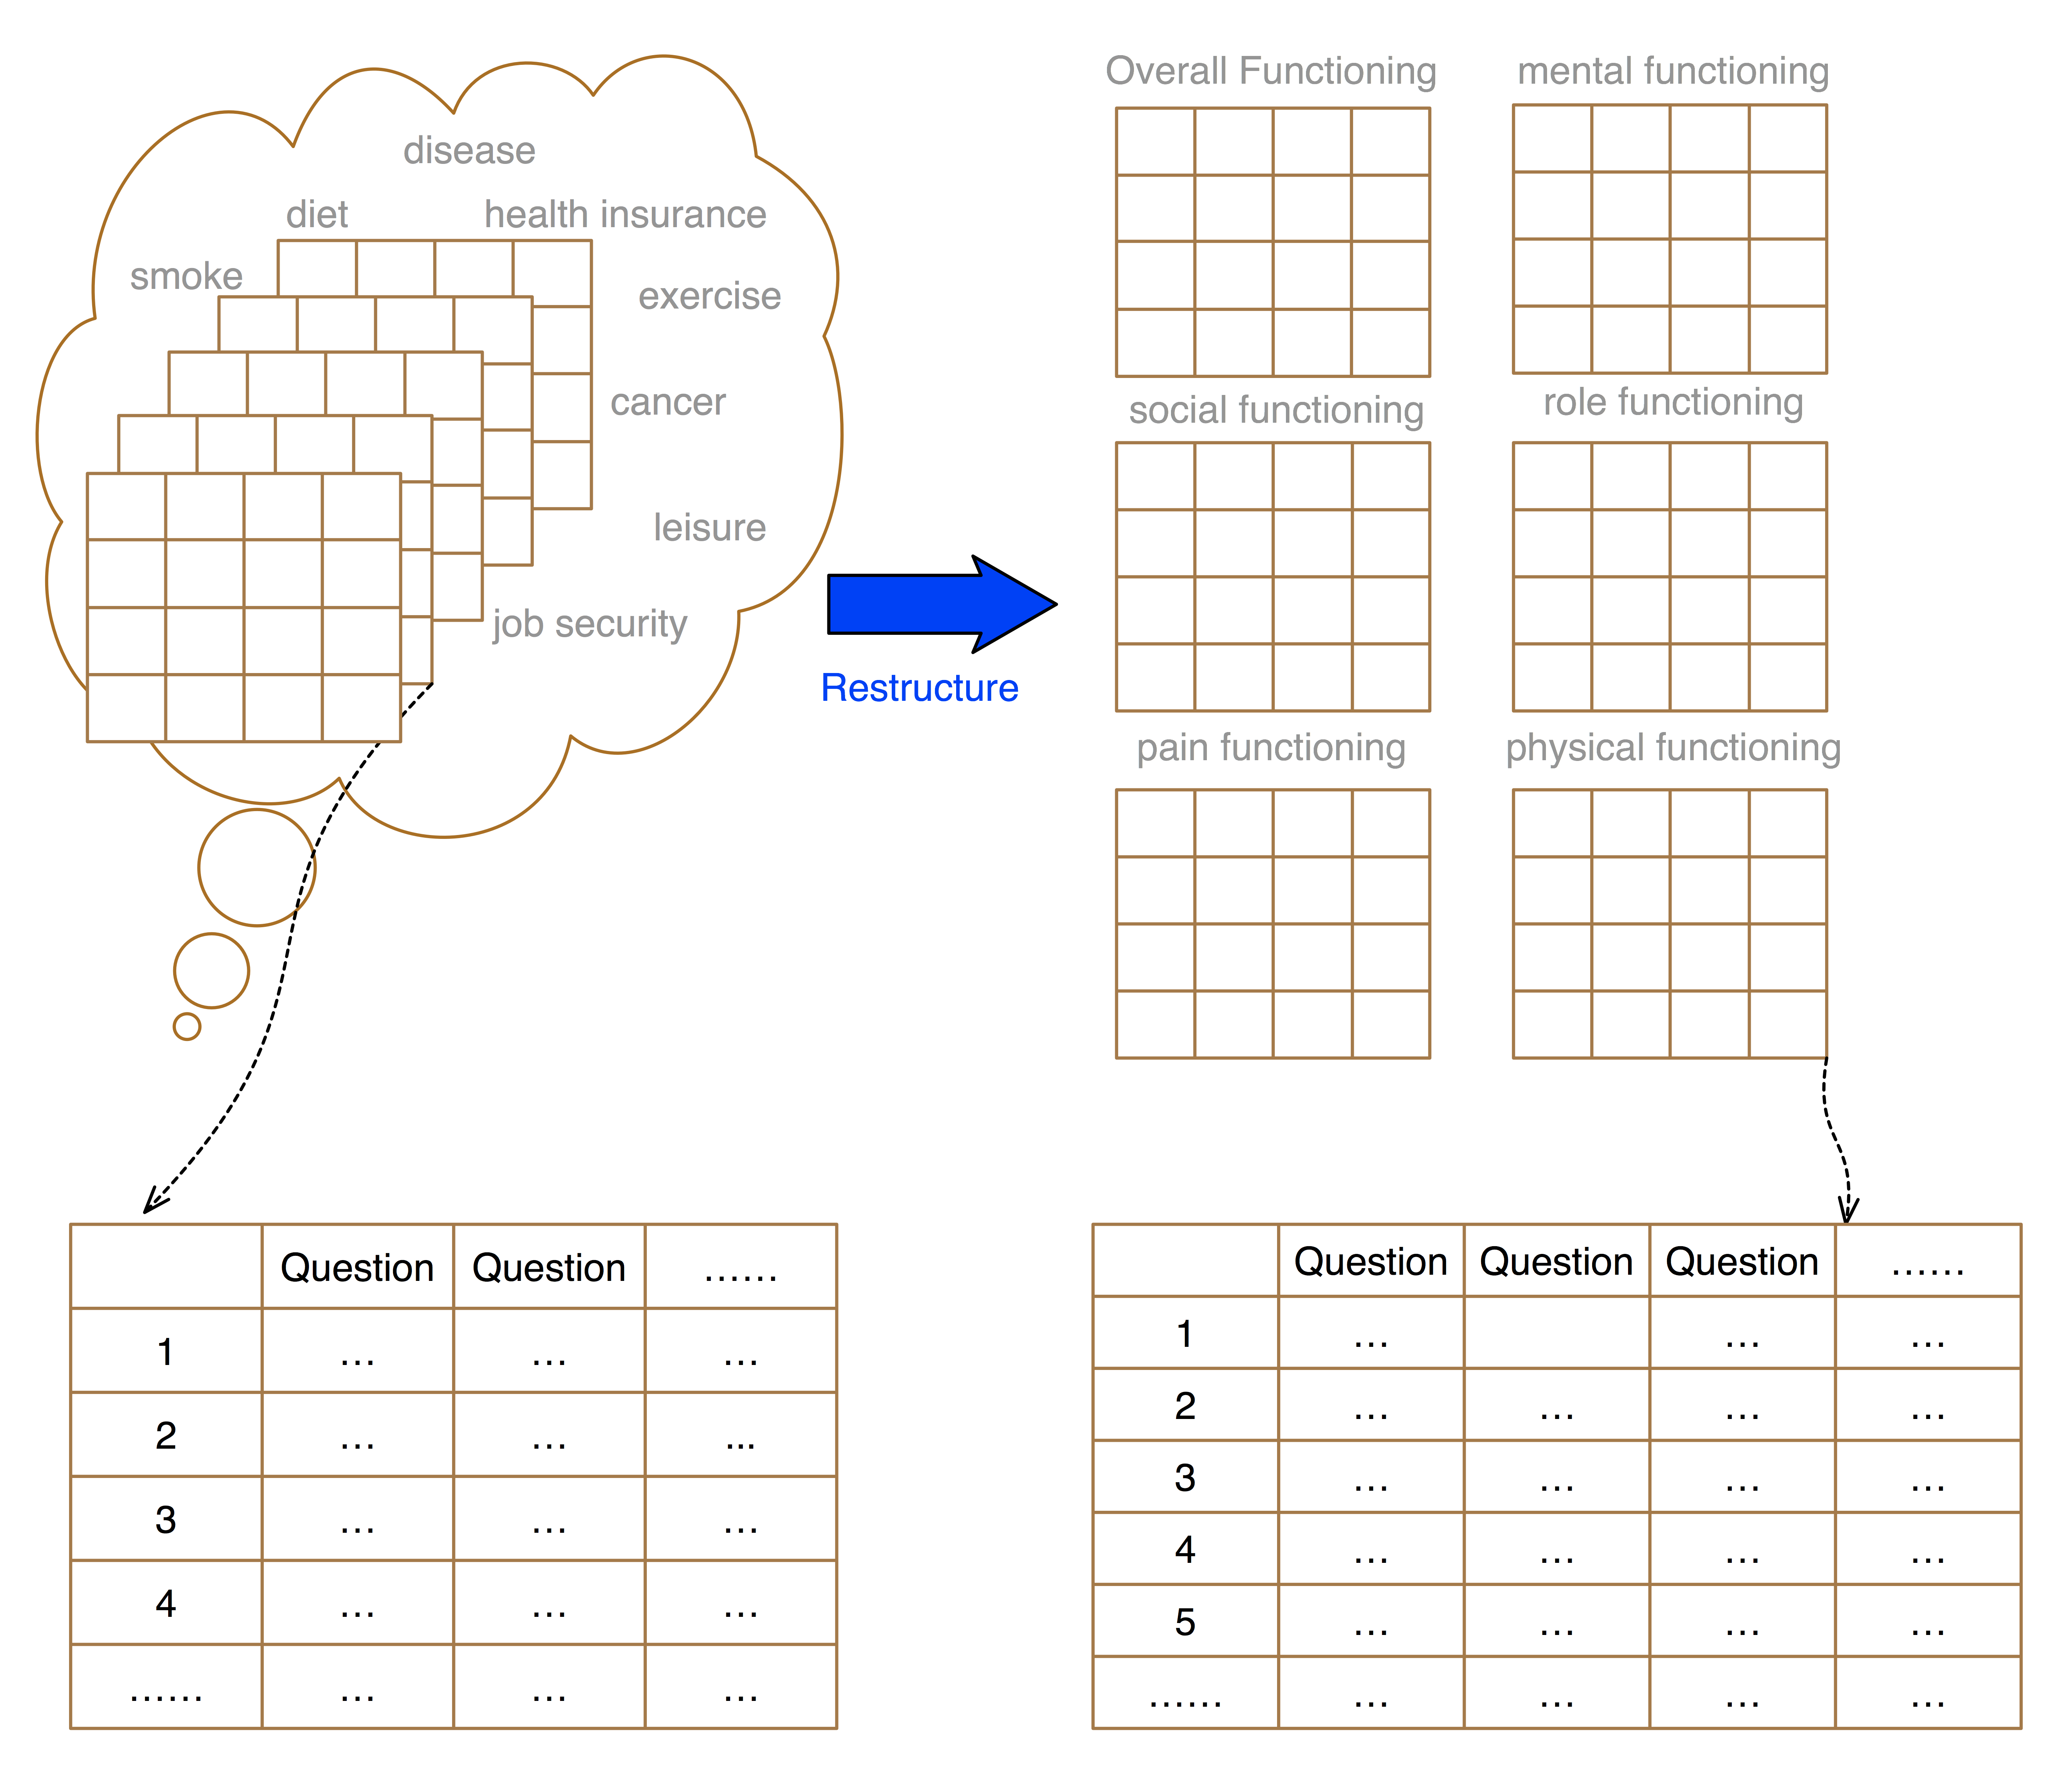
\includegraphics[width=0.6\textwidth]{restructure.png}
\caption{Data Restructure based on Psychological Knowledge Base} \label{fig2}
\end{figure}
%
%
%
%
%
%
%
%
%
%
\subsection{Modelling}
%
\subsubsection{4.4.1. Design ensemble}
In this study, we use an ensemble classification approach to build the model for detecting depression. It implements the independent ensemble methodology which applies several classification techniques in parallel. They are Decision Tree (DT) method, K-Nearest Neighbour (KNN) method, Naive Bayes (NB) algorithm and Support Vector Machine (SVM) technique. Each composite classifier among them is trained on the same portion of the training set in one run. The performance of them are evaluated by k-fold cross validation algorithm. And amalgamating all outputs of composite classifiers into a single prediction, we consequently generates the ensemble classifier. The main idea of this ensemble classification approach is to collect various outputs of multiple independent classifiers and combines them to improve the predictive performance. 
%
\subsubsection{4.4.2. Why ensemble}
In general, the ensemble method provides higher accuracies and better predictive performance than a single algorithm [Rokach]. There are several reasons why ensemble methods having a better performance [Sagi]: 
\renewcommand\labelitemii{$\square$}
\begin{itemize}
  \item Overfitting avoidance: "Averaging different hypothesis reduces the risk of choosing an incorrect hypothesis and therefore, improves the overall predictive performance."
  \item Computational advantage: "By combining several learners, ensemble methods decrease the risk of obtaining a local minimum."
  \item Strong Representation: "By combining different models, the search space may be extended and hence, a better fit to the data space is achieved. "
\end{itemize}
Moreover, ensemble methods are considered the potential solution for several machine learning challenges like class imbalance, concept drift and curse of dimensionality [Sagi]. For example, [Liu, Wang]most of the studies overlook a fundamental issue that is widely seen in real-world Twitter data, i.e., the class imbalance problem. To address the problem, we propose an ensemble learning approach, which involves three steps. In the first step, we adjust the class distribution in the imbalanced data set using various strategies, including random oversampling, random under-sampling and fuzzy-based oversampling. In the next step, a classification model is built upon each of the redistributed data sets. In the final step, a majority voting scheme is introduced to combine all the classification models. Experimental results obtained using real-world Twitter data indicate that the proposed approach can significantly improve the spam detection rate in data sets with imbalanced class distribution. And [concept drift]. Also, [curse of dimensionality].
%
Ensemble methods imitate human nature by seeking various solutions before making a final decision [Sagi] and therefore, it improves the overall performance in classification. 
%
%
%
%
\subsubsection{4.4.3. for each method, give technical purpose}
Our ensemble modelling involves several different classification methods. While more specifically each independent sub-model is trained, more targeted concepts is covered by the ensemble classifier and more accuracy it becomes. The first base model adopts Support Vector Machine algorithm. 
%
%
	\paragraph{Support Vector Machine (SVM)}
%
%
	\paragraph{Decision Tree (DT)}
%
%
	\paragraph{K-Nearest Neighbour (KNN)}
%
%
	\paragraph{Naive Bayes (NB) }
%
%
%
\subsubsection{4.4.4. Model}
%
%
\paragraph{4.4.4.1 performance weighting}
In order to combine all base classifiers' outputs, our modelling procedure adopts weighting ensemble method. Weighting ensemble method is very genetic when all base classifiers have uniform comparable outputs. The weight of each classifier can be set proportional to its accuracy performance on a validation set [Rokach]:\\
\begin{equation}\label{reio}
	w_{i} = \frac{1 - E_{i} }{\sum_{k = 1}^{n} (1 - E_{k}) } 
\end{equation}
where $E_{i} $ is a normalisation factor which is based on the predictive performance of classifier $i$ on the validation set. 
%
%
%
%
\paragraph{4.4.4.2 ensemble classifier}
In view of the fact that the ensemble classifier combines weighted outputs of all base classifiers, we can define the ensemble classifier as below: \\
\textbf{Definition 5} \textit{ Let the ensemble classifier \\
\begin{equation}\label{reio}
	\mathbb{M}_{e} = \sum_{k = 1}^{n} w_{i} M_{i} 
\end{equation}
where
\begin{itemize}
  \item $M_{i}$ presents a single base model;
  \item $w_{i}$ presents the weighting metric of predictive performance at specific base model $M_{i}$;
  \item $k$ is the order of base models;
  \item $n$ is the total number of base models, and in our case $n = 4$;
  \item $i$ is the order number of specific base model.
\end{itemize}
}
%
%
\subsubsection{4.4.5. Algorithm}
%
Given a health dataset of n examples and m features \\
$\mathbb{D}$ = $\mathbb{D}_{mental} + \mathbb{D}_{social} + \mathbb{D}_{role} + \mathbb{D}_{pain} + \mathbb{D}_{physical} + \mathbb{D}_{overall}$ = $\displaystyle \sum_{k=1, g \in Z}^{k=6, g \in Z}  \big\{ (x_{i, j}, y_{i, j}) \big\}$, \\ where 
 \begin{itemize}
 	\item $ x_{i, j} \in R^{m_{i}}, y_{i, j} = \{0, 1\}$, 
 	\item $\displaystyle \sum_{k=1}^{6}m_{i} = m$ , 
	\item $ |\mathbb{D}| $= $|\mathbb{D}_{mental}|$ = $|\mathbb{D}_{social}|$ = $|\mathbb{D}_{role}|$ = $|\mathbb{D}_{pain}| $= $|\mathbb{D}_{physical}|$ = $|\mathbb{D}_{overall}| =  n$.
 \end{itemize}
%
%
\IncMargin{1em}
\begin{algorithm}
	\SetKwData{Left}{left}\SetKwData{This}{this}\SetKwData{Up}{up}
	\SetKwFunction{Union}{Union}\SetKwFunction{FindCompress}{FindCompress}
	\SetKwInOut{Input}{input}\SetKwInOut{Output}{output}
		\Input{$\mathbb{D}$ = $\mathbb{D}_{mental} + \mathbb{D}_{social} + \mathbb{D}_{role} + \mathbb{D}_{pain} + \mathbb{D}_{physical} + \mathbb{D}_{overall}$}
		\Output{the ensemble classifier}
		\BlankLine
		\emph{special treatment of the first line}\;
		\lForEach{element $e$ of the line $i$}{\FindCompress{p}}
	\caption{Ensemble}\label{algo_disjdecomp}
\end{algorithm}
\DecMargin{1em}
%
%
%
%
%
%
%
%
%
%
%
%
%
%
%
%
%
%
%
%
%
\pagebreak
\section{Experiment}

\subsection{Experiment Design}

\subsection{Dataset}

\subsection{Baseline Models}

\subsection{Performance Measure}
\paragraph{5.4.1 Predictive Performance of Base Classifier}
The predictive performance of each base classifier in our model is evaluated by F1 score which is generated on confusion matrix of validation. In confusion matrix, we simply let the number of real mental healthy cases in the training set as \textbf{condition positive (P)} and let the number of real depressive cases in the training set as  \textbf{condition negative (N)}. And four derivations are defined to make it clear if the classifier is confusing binary classes (P and N):  \\
\begin{enumerate}[label=(\roman*)]
\item let the number of cases where the classifier correctly predicts P as \textbf{ true positive (TP)}
\item let the number of cases where the classifier correctly predicts N as \textbf{true negative (TN)}
\item let the number of cases where the classifier incorrectly predicts P as \textbf{false positive (FP)}
\item let the number of cases where the classifier incorrectly predicts N as \textbf{false negative (FN)}
\end{enumerate}
And four following terminologies are hence defined as below:
\begin{enumerate}[label=\alph*)]
\item \textbf{ Recall or True Positive Rate (TPR)}: \\ 
		\begin{center} $\displaystyle TPR = \frac{TP}{TP + FN} $ \end{center}
\item \textbf{Specificity or True Negative Rate (TNR)}: \\ 
		\begin{center} $\displaystyle TNR = \frac{TN}{TN + FP} $ \end{center}
\item \textbf{Precision or Positive Predictive Value (PPV)}: \\
		\begin{center} $\displaystyle PPV = \frac{TP}{TP + FP} $ \end{center}
\item \textbf{Accuracy (ACC)}: \\ 
		\begin{center} $\displaystyle ACC = \frac{TP + TN}{TP + TN + FP + FN} $ \end{center}
\end{enumerate}
F1 score is a balanced measure of both the precision (PPV) and the recall (TPR) of the validation: 
\begin{equation}\label{reio}
	F1 = \frac{2 }{\frac{1}{TPR} + \frac{1}{PPV}} = \frac{2TP}{2TP + FP + FN}
\end{equation}
Referred to normalisation factor $E$ in equation (1), F1 score need to be normalised first and then is applied to equation (1) to calculate the weight fo each base classifier. 
%
%
%
%
%
%
%
%
%
%
%
%
%
%
%
%
%
%
%
%
%
%
\pagebreak
\section{Results and Discussions}
\subsection{Experimental Results}
\subsection{Discussions}
%
%
%
%
%
%
%
%
%
%
%
%
%
%
%
%
%
%
%
%
%
\pagebreak
\section{Analysis}
\subsection{Sensitivity Study}
%
%
%
%
%
%
%
%
%
%
%
%
%
%
%
%
%
%
%
%
%
\pagebreak
\section{Conclusion and Future Work}
%
%
% ---- Bibliography ----
%
\pagebreak
\begin{thebibliography}{8}
%\bibitem{ref_article1}		
%
\bibitem{ref_article}	R. L. Spitzer, K. Kroenke, and J. B. Williams, "Validation and utility of a self-report version of PRIME-MD: the PHQ primary care study. Primary Care Evaluation of Mental Disorders. Patient Health Questionnaire," JAMA, vol. 282, no. 18, pp. 1737-44, Nov 10 1999.
%
\bibitem{ref_article}	K. Kroenke, R. L. Spitzer, and J. B. Williams, "The PHQ-9: validity of a brief depression severity measure," J Gen Intern Med, vol. 16, no. 9, pp. 606-13, Sep 2001.
%
\bibitem{ref_article}	M. Résibois, P. Kuppens, I. Van Mechelen, P. Fossati, and P. Verduyn, "Depression severity moderates the relation between self-distancing and features of emotion unfolding," Personality and Individual Differences, vol. 123, pp. 119-124, 2018.
%
\bibitem{ref_article}	B. T. Stegenga et al., "Depression, anxiety and physical function: exploring the strength of causality," Journal of Epidemiology and Community Health, vol. 66, no. 7, pp. e25-e25, 2012.
%
\bibitem{ref_article}	H. Xiao, J. Y. Yoon, and B. Bowers, "Living Arrangements and Quality of Life," Western Journal of Nursing Research, vol. 38, no. 6, pp. 738-752, 2015.
%
%
\bibitem{ref_article} Rokach, L.: ‘Ensemble-based classifiers’, Artificial Intelligence Review, 2010, 33, (1), pp. 1-39.
%
%
%
%
%
%
%
%
%
%
%
%
%
%
%
%
\end{thebibliography}
\end{document}
